\documentclass[../../main.tex]{subfiles}
\begin{document}

\begin{flushright}
  \footnotesize\textit{【自動文字起こし・要確認】}
\end{flushright}

{\bf [解答]}
点$X$に対し$\overrightarrow{AX}=\vec{x}$とおく．$\vec b=\overrightarrow{AB}$，$\vec d=\overrightarrow{AD}$は互いに一次独立である．

\begin{align}
  \vec e=\dfrac{1}{2}\vec b，\quad \vec f=\vec b+\dfrac{2}{3}\vec d，\quad \vec g=\dfrac{1}{4}\vec b+\vec d
\end{align}

から，$s,t\in\mathbb{R}$として
\begin{align}
  \vec p&=s\vec e+(1-s)\vec c=\dfrac{1}{2}s\vec b+(1-s)(\vec b+\vec d)=\left(1-\dfrac{1}{2}s\right)\vec b+(1-s)\vec d，\\
  \vec p&=t\vec f+(1-t)\vec g=t\left(\vec b+\dfrac{2}{3}\vec d\right)+(1-t)\left(\dfrac{1}{4}\vec b+\vec d\right)=\left(\dfrac{1}{4}+\dfrac{3}{4}t\right)\vec b+\left(1-\dfrac{1}{3}t\right)\vec d
\end{align}

とおける（$\vec c=\overrightarrow{AC}=\vec b+\vec d$）．係数比較して
\begin{align}
  1-\dfrac{1}{2}s=\dfrac{1}{4}+\dfrac{3}{4}t，\qquad 1-s=1-\dfrac{1}{3}t
\end{align}
\begin{align}
  \therefore\ t=\dfrac{9}{11}，\quad s=\dfrac{3}{11}
\end{align}

だから
\begin{align}
  \vec p=\dfrac{19}{22}\vec b+\dfrac{8}{11}\vec d
\end{align}

とおける．$k,\ell\in\mathbb{R}$として
\begin{align}
  \vec q=\vec b+k\vec d=\ell\left(\dfrac{19}{22}\vec b+\dfrac{8}{11}\vec d\right)
\end{align}

とおける．係数比較して$\ell=\dfrac{22}{19}$だから，$|AP|:|PQ|=19:3$．

\begin{figure}[htb]
  \centering
  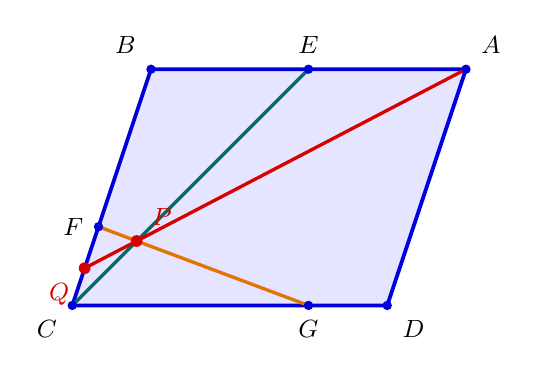
\begin{tikzpicture}[scale=1.0, >=stealth,
    every node/.style={font=\small}]
    \coordinate (A) at (4,3);
    \coordinate (B) at (0,3);
    \coordinate (C) at (-1,0);
    \coordinate (D) at (3,0);
    \coordinate (E) at (2,3);
    \coordinate (F) at (-0.666667,1);
    \coordinate (G) at (2,0);
    % P=CE∩FG，Q=AP∩BC を本文の係数比較に合わせて配置．
    \coordinate (P) at (-0.181818,0.818182);
    \coordinate (Q) at (-0.842105,0.473684);
    \fill[blue!10] (A)--(B)--(C)--(D)--cycle;
    \draw[blue!85!black, line width=1.35pt]
    (A)--(B)--(C)--(D)--cycle;
    \draw[teal!85!black, line width=1.2pt] (C)--(E);
    \draw[orange!90!black, line width=1.2pt] (F)--(G);
    \draw[red!85!black, line width=1.2pt] (A)--(Q);
    \foreach \point/\position in {
      A/above right,B/above left,C/below left,D/below right,
    E/above,F/left,G/below} {
      \node[circle, fill=blue!85!black, inner sep=1.2pt] at (\point) {};
      \node[\position=2pt] at (\point) {$\point$};
    }
    \node[circle, fill=red!85!black, inner sep=1.5pt] at (P) {};
    \node[circle, fill=red!85!black, inner sep=1.5pt] at (Q) {};
    \node[above right=2pt, red!85!black] at (P) {$P$};
    \node[below left=2pt, red!85!black] at (Q) {$Q$};
  \end{tikzpicture}
  \caption{平行四辺形$ABCD$と点$E$，$F$，$G$，$P$，$Q$の位置関係}
\end{figure}

\newpage

\end{document}
